% widom-atlas v0.6 --- standalone report.
% Reuses the v3 manuscript preamble + float-placement discipline.
\documentclass[11pt,a4paper]{article}

\usepackage[utf8]{inputenc}
\usepackage[T1]{fontenc}
\usepackage{lmodern}
\usepackage{amsmath,amssymb}
\usepackage{textcomp}
\usepackage{array}
\usepackage{booktabs}
\usepackage{longtable}
\usepackage{graphicx}
\usepackage{xcolor}
\usepackage[margin=1in]{geometry}
\usepackage[hidelinks]{hyperref}
\usepackage{caption}
\usepackage{microtype}
\usepackage{placeins}
\usepackage{calc}
\usepackage{needspace}
\setlength{\emergencystretch}{3em}
\graphicspath{{figures/}}

% pandoc-fragment macros (normally provided by pandoc's full template)
\providecommand{\real}[1]{#1}
\providecommand{\tightlist}{\setlength{\itemsep}{0pt}\setlength{\parskip}{0pt}}

% --- Unicode safety for pdflatex (every glyph used in the transpiled body) ---
\DeclareUnicodeCharacter{2212}{\ensuremath{-}}        % minus
\DeclareUnicodeCharacter{00D7}{\ensuremath{\times}}   % times
\DeclareUnicodeCharacter{00B7}{\ensuremath{\cdot}}    % middle dot
\DeclareUnicodeCharacter{2248}{\ensuremath{\approx}}
\DeclareUnicodeCharacter{2192}{\ensuremath{\rightarrow}}
\DeclareUnicodeCharacter{27E8}{\ensuremath{\langle}}
\DeclareUnicodeCharacter{27E9}{\ensuremath{\rangle}}
\DeclareUnicodeCharacter{0394}{\ensuremath{\Delta}}
\DeclareUnicodeCharacter{03B4}{\ensuremath{\delta}}
\DeclareUnicodeCharacter{03B2}{\ensuremath{\beta}}
\DeclareUnicodeCharacter{03C3}{\ensuremath{\sigma}}
\DeclareUnicodeCharacter{03B5}{\ensuremath{\varepsilon}}
\DeclareUnicodeCharacter{03BC}{\ensuremath{\mu}}
\DeclareUnicodeCharacter{03B1}{\ensuremath{\alpha}}
\DeclareUnicodeCharacter{00B2}{\ensuremath{^2}}
\DeclareUnicodeCharacter{00B3}{\ensuremath{^3}}
\DeclareUnicodeCharacter{2264}{\ensuremath{\le}}
\DeclareUnicodeCharacter{2265}{\ensuremath{\ge}}
\DeclareUnicodeCharacter{226B}{\ensuremath{\gg}}
\DeclareUnicodeCharacter{226A}{\ensuremath{\ll}}
\DeclareUnicodeCharacter{221E}{\ensuremath{\infty}}
\DeclareUnicodeCharacter{2261}{\ensuremath{\equiv}}
\DeclareUnicodeCharacter{00C5}{\AA{}}                 % Angstrom
\DeclareUnicodeCharacter{2080}{\ensuremath{_0}}
\DeclareUnicodeCharacter{2081}{\ensuremath{_1}}
\DeclareUnicodeCharacter{2082}{\ensuremath{_2}}
\DeclareUnicodeCharacter{2083}{\ensuremath{_3}}
\DeclareUnicodeCharacter{2074}{\ensuremath{^4}}
\DeclareUnicodeCharacter{2077}{\ensuremath{^7}}
\DeclareUnicodeCharacter{207B}{\ensuremath{^{-}}}
\DeclareUnicodeCharacter{2070}{\ensuremath{^0}}
\DeclareUnicodeCharacter{2076}{\ensuremath{^6}}
\DeclareUnicodeCharacter{2009}{\,}                    % thin space
\DeclareUnicodeCharacter{2011}{-}                     % non-breaking hyphen
\DeclareUnicodeCharacter{2086}{\ensuremath{_6}}
\DeclareUnicodeCharacter{21D2}{\ensuremath{\Rightarrow}}
\DeclareUnicodeCharacter{2705}{\ensuremath{\checkmark}}   % done
\DeclareUnicodeCharacter{274C}{\ensuremath{\times}}       % not done
\DeclareUnicodeCharacter{00A7}{\S}
\DeclareUnicodeCharacter{00B9}{\ensuremath{^1}}

\title{widom-atlas v0.6: Cross-engine Validation and MLIP\\
Out-of-Distribution Governance for Widom-Insertion\\
Adsorption on the kUPS Engine}
\author{Onur Alexander William Aydogan\\
Waynestark Enterprises Limited}
\date{}

\begin{document}
\maketitle

\begin{abstract}
\noindent A published force-field parameter table is not a complete simulation recipe: the load-bearing
ingredients (a short-range protection convention, a mixing rule on the framework atoms, a dispersion
correction, an LJ truncation convention) are often unpublished, and an ungoverned pipeline that guesses
any of them wrong returns a confident, wrong number with no warning. \textbf{widom-atlas} does not
re-estimate adsorption; it locks the complete recipe behind a number, checks cross-engine parity and
convergence, detects out-of-distribution insertions, and \emph{refuses} averages built on unphysical
configurations. This v0.6 report demonstrates that domain-of-validity / realization-gap failure class
end-to-end on CuspAI's JAX engine \textbf{kUPS} and on the machine-learning interatomic potential
(MLIP) kUPS ships. Auditing its own positive control surfaced a headline catch: the originally-locked
all-silica MFI + Ar recipe \emph{double-counted silicon} --- Talu--Myers' Ar--O cross-parameter already
folds silicon's dispersion into oxygen, and the locked recipe added an explicit Ar--Si on top --- so it
landed inside the strict band only as a fortuitous cancellation of four compounding errors --- a coincidence, not a coherent result; rebuilt clean (pure Talu oxygen-only,
converged convention, on Talu's calibration Olson geometry) it reproduces the corrected reference
$K_H = 0.200$ exactly and cross-engine (native 0.200, RASPA3 0.199). Separately and intact: to our
knowledge and per public-source searches conducted on 15 June 2026, the first published independent
cross-engine validation of kUPS's Widom estimator (isosteric
heat reproduced to 0.01--0.22 kJ/mol on two locked controls; independent estimators agree on the shared
recipe to 1.1\% on $K_H$, the dominant $K_H$ convention gaps traced to named truncation/shift
conventions, with one normalization-flavoured residual on the electrostatic control flagged open), and a
four-configuration MLIP out-of-distribution governance demonstration that discriminates two failure
modes, screen-passes a dispersion-corrected route, and respects the model's training domain. \textbf{The
evidence base is the version-controlled repository state: every number in this document traces to
committed JSON and regenerates from the figure scripts.}
\end{abstract}

\section{Thesis}\label{thesis}

A published force-field parameter table is \textbf{not} a complete
simulation recipe. The load-bearing ingredients are frequently
unpublished: a short-range protection convention, a mixing rule applied
to the framework atoms, a dispersion correction, a blocking radius, an
energy-reference convention. An ungoverned pipeline that guesses any of
them wrong returns a confident, wrong number with no warning. This is
the \textbf{domain-of-validity / realization-gap} failure class.
The v0.4/v0.4.2 classical audit established this failure class on locked
classical force-field recipes; \textbf{v0.6 retargets the same governance
logic onto CuspAI's own engine (kUPS) and the machine-learning
interatomic potential (MLIP) it ships} --- and shows a governance
layer that \emph{characterizes, discriminates, and where the evidence
supports it, screen-passes a governed remediation.}

\textbf{Reader note on labels.} Branch codes such as \texttt{6c} and
\texttt{4c} are internal locked-recipe identifiers, not chemical formulae
or universal benchmark names: each fixes one complete Widom-insertion
recipe (structure, guest model, force field, charges, mixing rule,
electrostatics, backend, sampling, and reference). Branch 6c is the
all-silica MFI + Ar recipe used as the positive control; branch 4c is the
Si-CHA + CO\textsubscript{2} charged-zeolite control. ``Native'' is this
project's own independent Python Widom estimator (not a generic term),
reported alongside the external Monte Carlo engine RASPA3. The version
labels are internal repository milestones: v0.4 and v0.4.2 are the locked
and corrected classical-audit layers, v0.5 is non-load-bearing
consolidation or extension material, and v0.6 is this kUPS and MLIP
governance extension.

Three results carry the report: 1. \textbf{A2/F1} --- the originally-locked positive
control \emph{double-counted silicon}; its strict-band agreement was a fortuitous four-error
cancellation; rebuilt clean (single-source, Talu's calibration Olson
geometry) it reproduces the corrected reference \(K_H = 0.200\)
cross-engine (native 0.200, RASPA3 0.199) (Finding~F1). 2. \textbf{A2-F2} --- to our knowledge, the first published
independent validation of kUPS's (six-week-old, unreleased) Widom
estimator. 3. \textbf{WPB} --- a four-configuration MLIP demonstration:
discriminate two failure modes, screen-pass a dispersion-corrected
route, and show the failure generalizes across MLIP families.

\begin{center}\rule{0.5\linewidth}{0.5pt}\end{center}

\section{Cross-engine Widom parity
(WPA-A2)}\label{cross-engine-widom-parity-wpa-a2}

\subsection{System and recipe}\label{system-and-recipe}

6c positive control: \textbf{MFI (all-silica) + Ar} at \(T = 298.15\) K,
TraPPE-zeo (Bai 2013) framework + Talu--Myers 2001 Ar--O cross-pair. The
framework attribution is stated here as TraPPE-zeo to match the recipe
table below; an earlier draft of this section credited the framework to
García-Pérez 2007, which the table never supported. The complete locked
recipe (recovered verbatim from the RASPA3 evidence
\texttt{force\_field.json}):

{%
\needspace{12\baselineskip}
\begin{longtable}[]{@{}lll@{}}
\toprule\noalign{}
element & self LJ (ε/K, σ/Å) & source \\
\midrule\noalign{}
\endhead
\bottomrule\noalign{}
\endlastfoot
Ar & 119.8 / 3.405 & Talu-Myers 2001 \\
O & 53.0 / 3.3 & TraPPE-zeo, Bai 2013 \\
Si & 22.0 / 2.3 & TraPPE-zeo, Bai 2013 \\
\end{longtable}
}

Ar--O is an \textbf{explicit} binary (93.0 K / 3.335 Å, Talu-Myers);
\textbf{MixingRule Lorentz-Berthelot}, \textbf{truncation shifted},
cutoff 12 Å, \textbf{TailCorrections false}, no electrostatics.
Critically, the Lorentz-Berthelot rule applied to the framework
self-parameters generates a \textbf{second} interaction ---
\textbf{Ar--Si (51.34 K / 2.8525 Å)} --- in addition to the explicit
Ar--O term. This is the \emph{as-locked} recipe, recorded verbatim;
Finding~F1 (§2.4) shows this Ar--Si term is a \emph{silicon double-count}
(Talu's Ar--O already folds silicon's dispersion into oxygen) and gives
the clean single-source rebuild that reproduces the corrected reference.

\subsection{The clean metric}\label{the-clean-metric}

Engines report different units (kUPS: K\_H in ų/eV; RASPA3/native:
mol·kg⁻¹·bar⁻¹), so the comparison is on the engine-agnostic
\textbf{⟨exp(−βU)⟩}, with K\_H and q\_st reported in common units.

\subsection{Result}\label{result}

{%
\needspace{12\baselineskip}
\begin{longtable}[]{@{}
  >{\raggedright\arraybackslash}p{(\linewidth - 6\tabcolsep) * \real{0.2500}}
  >{\raggedright\arraybackslash}p{(\linewidth - 6\tabcolsep) * \real{0.2500}}
  >{\raggedright\arraybackslash}p{(\linewidth - 6\tabcolsep) * \real{0.2500}}
  >{\raggedright\arraybackslash}p{(\linewidth - 6\tabcolsep) * \real{0.2500}}@{}}
\toprule\noalign{}
\begin{minipage}[b]{\linewidth}\raggedright
Engine (full recipe unless noted)
\end{minipage} & \begin{minipage}[b]{\linewidth}\raggedright
⟨W⟩
\end{minipage} & \begin{minipage}[b]{\linewidth}\raggedright
K\_H (mol·kg⁻¹·bar⁻¹)
\end{minipage} & \begin{minipage}[b]{\linewidth}\raggedright
q\_st (kJ/mol)
\end{minipage} \\
\midrule\noalign{}
\endhead
\bottomrule\noalign{}
\endlastfoot
RASPA3 (locked reference) & --- & \textbf{0.2070} & \textbf{16.03} \\
native independent (Ar--O \textbf{+ Ar--Si}) & 9.54 & \textbf{0.2093}
(+1.1 \%) & 15.91 (−0.12) \\
kUPS Widom (Ar--O \textbf{+ Ar--Si}) & 11.08 & 0.2432 (+16.2 \%) & 16.25
(+0.22) \\
native (Ar--O \textbf{only}, naive) & 5.24 & 0.1149 (\textbf{1.8× low})
& 14.36 \\
kUPS (Ar--O only) & 5.98 & 0.1313 & --- \\
\end{longtable}
}

{\footnotesize\noindent Percent differences are relative to the stated comparator. The native
\(K_H\) offset (\(+1.1\,\%\)) is relative to the RASPA3 locked reference; the kUPS \(K_H\) offset
(\(+16.2\,\%\)) is quoted relative to the convention-matched native shifted estimator when discussing
the shifted-versus-truncated convention gap (it is \(+17.5\,\%\) relative to RASPA3). The \(q_{st}\)
offsets in parentheses are relative to RASPA3.\par}

\subsection{Finding F1 --- a silicon double-count caught by audit (and a
clean rebuild)}\label{finding-f1-the-arsi-term-is-load-bearing-1.82-on-k_h}

The originally-locked 6c recipe \textbf{double-counted silicon}, and
agreed with its reference only as a fortuitous cancellation of four
compounding errors. Talu--Myers' Ar--O cross-parameter (93.0 K) is the
Lorentz--Berthelot combination of argon with an oxygen-only
\emph{effective} oxygen (72.2 K, Talu Table 1) that already folds
silicon's dispersion into oxygen --- Talu's model is oxygen-only by
construction (Talu \S2: ``ignores partially concealed silicon atoms and
lumps their dispersion energy with the oxygen atoms''). The locked recipe
nonetheless added an explicit Ar--Si from an active TraPPE-zeo framework
silicon, counting silicon twice (\(\times 1.82\) on \(K_H\)). That
spurious term compensated three further errors --- an idealized (IZA)
rather than the calibration (Olson) geometry (\(\sim\!-25\,\%\)), an
under-converged 12~\AA{} tail-off cutoff (\(\sim\!-25\,\%\) more), and a
reference value mis-derived by \(\sim\!12\,\%\) (0.224 vs the correct
0.200) --- which multiplied back to roughly the (wrong) reference.
Removing all four and running the coherent \textbf{single-source} recipe
(pure Talu, oxygen-only, no Ar--Si) at a converged cutoff on Talu's own
(Olson) geometry reproduces the \textbf{corrected} reference
(\(K_H = 0.200\)) exactly and \textbf{cross-engine}: native 0.200,
RASPA3 0.199 (parity 0.5\,\%), \(q_{st}\) 14.97 (within 0.7 kJ/mol of
calorimetry). In strict-band terms the as-locked hybrid lands in-band against \emph{both} the
mis-derived 0.224 and the corrected 0.200 reference; the rebuild changes the recipe's coherence, not the
pass/fail verdict.

{%
\needspace{12\baselineskip}
\begin{longtable}[]{@{}lll@{}}
\toprule\noalign{}
6c recipe / setup & \(K_H\) (mol/kg/bar) & note \\
\midrule\noalign{}
\endhead
\bottomrule\noalign{}
\endlastfoot
locked hybrid (IZA, 12~\AA{} tail-off) & 0.207 & in-band by a fortuitous cancellation (also passes 0.200) \\
\(-\) double-counted silicon & 0.115 & pure Talu, oxygen-only (IZA, 12~\AA{}) \\
\(+\) converged 24~\AA{} + tail & 0.154 & numerical defect fixed (IZA) \\
\(+\) Olson calibration geometry & \textbf{0.200} & native; RASPA3 0.199 (parity 0.5\,\%) \\
\textbf{corrected reference} (Dunne 1996) & \textbf{0.200} & strict window [0.159, 0.252] \\
structure sensitivity (single-source) & 0.200 / 0.205 / 0.154 & Olson / van Koningsveld / IZA \\
\end{longtable}
}

(The locked hybrid evidence is retained intact as the documented
negative case.)

\subsection{Finding F2 --- independent cross-engine validation of
kUPS's Widom estimator}\label{finding-f2-the-first-published-independent-validation-of-kupss-widom-estimator}

kUPS ships a Widom test-particle module (\texttt{kups.mcmc.widom}; present
in the source \texttt{main} branch, absent from the released PyPI
\texttt{kups\ 1.0.1}; no published external validation). \emph{Version
pinning.} The module was read and exercised from the public source
repository as obtained on 15 June 2026; because it is not in any tagged
release, the artefact validated here is a moving target unless pinned,
and any reader reproducing this section should record the commit they
obtained. This is a stated limitation of F2, by this report's own
reproducibility criterion. We make no priority claim: we are simply
\emph{not aware} of a prior external check of this specific module ---
as distinct from standalone Widom packages (e.g.\ the
\texttt{widom} ASE add-on) and from machine-learned-potential adsorption
benchmarks such as ODAC25 (Sriram et al.\ 2025, arXiv:2508.03162), based on public-source
searches (the kUPS source carries internal unit tests only; the open
tracker was inspected 2026-06-12 --- one unrelated feature issue).

\begin{itemize}
\item
  \textbf{The estimator is correct.} \texttt{widom\_test()} returns lnα
  = −βΔU for a ghost insertion ⇒ \textbf{W ≡ exp(−βU)} --- identical to
  the textbook Widom weight; the μ\_ex / K\_H / q\_st reductions match
  widom-atlas's definitions. Verified by reading the source \emph{and}
  by the parity run.
\item
  \textbf{q\_st is validated to 0.22 kJ/mol} (16.25 vs 16.03 RASPA3;
  15.91 native). The energies are right.
\item
  \textbf{The +16 \% K\_H is a shifted-vs-truncated LJ convention ---
  root-caused, not a normalization bug.} kUPS's
  \texttt{lennard\_jones\_energy} is \textbf{truncated, not
  energy-shifted} (\texttt{4ε(c6²−c6)} masked at cutoff, no
  \texttt{−U(rc)} term); our config (\texttt{tail\_correction:\ false},
  no \texttt{truncation\_radius}) selects that plain variant. RASPA3's
  recipe is \texttt{TruncationMethod:\ shifted}, and the native
  estimator shifts too. The unshifted potential is more attractive by
  U(rc) per interaction. Toggling the shift off in native reproduces
  kUPS:

  {%
  \needspace{12\baselineskip}
  \begin{longtable}[]{@{}llll@{}}
  \toprule\noalign{}
  native (with-Si) & ⟨W⟩ & K\_H & q\_st (kJ/mol) \\
  \midrule\noalign{}
  \endhead
  \bottomrule\noalign{}
  \endlastfoot
  shifted (RASPA convention) & 9.54 & 0.2093 & 15.91 \\
  truncated / no-shift (kUPS convention) & 11.35 & 0.2490 & 16.34 \\
  kUPS Widom & 11.08 & 0.2432 & 16.25 \\
  \end{longtable}
  }

  The implied constant shift δ = RT·ln(11.35/9.54) = \textbf{0.43
  kJ/mol} (predicted ≈0.35) explains \textbf{both} the +16 \% K\_H
  \textbf{and} the +0.34 kJ/mol q\_st: matching kUPS's convention,
  native-no-shift agrees with kUPS to \textbf{+2.4 \% on K\_H (within
  the 3.4 \% SEM) and 0.09 kJ/mol on q\_st}. Neither engine is wrong ---
  but the shift convention is a load-bearing recipe element worth
  \textasciitilde16 \% on K\_H, which must be locked and matched. The
  exponential sensitivity of K\_H to a constant energy offset, and the
  resulting need to lock the tail/truncation convention, are established
  (Jablonka, Ongari \& Smit 2019, \emph{J. Chem. Theory Comput.}\ \textbf{15},
  5635; Dubbeldam et al.\ 2016, \emph{Mol. Simul.}\ \textbf{42}, 81). The
  magnitude is also analytically predictable from the Lennard-Jones tail
  integral and the framework atom density, which for MFI at a 12 Å cutoff
  gives \(\approx 0.4\) kJ/mol; our measured \(\delta \approx 0.43\) kJ/mol
  is therefore a \emph{cross-engine confirmation} of a known effect at the
  expected size, not a new one. Does
  \textbf{not} affect q\_st-as-physics or the OOD governance demo
  (energy path).
\end{itemize}

The recipe all three engines share for this parity is the as-locked
hybrid now reframed in F1 as a silicon double-count: F2 establishes that
independent estimators agree on a \emph{common} recipe (to \(1.1\,\%\) on
\(K_H\)), not that the recipe reproduces experiment --- that correction
lives entirely in F1, and the two findings are consistent.

\begin{center}\rule{0.5\linewidth}{0.5pt}\end{center}

\section{Blocking-sphere governance
(WPA-A3)}\label{blocking-sphere-governance-wpa-a3}

kUPS exposes the v0.5 short-range-protection lesson as an explicit API
--- \texttt{blocking\_spheres} (per-host hard-sphere exclusions). So the
convention is no longer a claim of ours; it is CuspAI's own engineering.
A sweep on the 6c system, with blocking spheres placed on 64 of the
192 framework-oxygen positions in the MFI cell (every third O, a
uniform one-in-three subsample chosen to cover the pore network without
tiling the whole framework):

{%
\needspace{12\baselineskip}
\begin{longtable}[]{@{}lllll@{}}
\toprule\noalign{}
blocking & radius (Å) & K\_H (ų/eV) & ΔK\_H & q\_st (kJ/mol) \\
\midrule\noalign{}
\endhead
\bottomrule\noalign{}
\endlastfoot
off & --- & 1.798×10⁷ & --- & 16.25 \\
on & 2.0 & 1.856×10⁷ & +3.2 \% & 16.34 \\
on & 3.0 & 1.812×10⁷ & +0.8 \% & 16.28 \\
\end{longtable}
}

\textbf{Finding.} On a physically-repulsive LJ recipe blocking is a
\textbf{no-op} (ΔK\_H \textless{} SEM, q\_st unchanged): the potential
already excludes overlaps, so a hard sphere on top adds nothing. The
corollary is the governance lesson --- \textbf{blocking is load-bearing
exactly when the recipe has an \emph{unphysical} short-range attraction
the potential does not repel} (open-metal-site over-binding; the v0.5 1b
exp-6 case). A recipe's blocking configuration is therefore part of the
recipe and must be locked: invisible on an all-silica LJ host, decisive
on an OMS host. The individual +0.8\ldots+3.2 \% \(K_H\) entries are
\textbf{not interpreted}: they are non-monotonic in the sphere radius
and both lie inside the quoted 3.4 \% SEM, so the correct reading of
this sweep is \emph{no measurable effect}, not a trend.

\begin{center}\rule{0.5\linewidth}{0.5pt}\end{center}

\section{MLIP out-of-distribution governance (WPB) --- the
headline}\label{mlip-out-of-distribution-governance-wpb-the-headline}

\subsection{Setup}\label{setup}

Widom insertions of \textbf{Ar into all-silica CHA}, N = 120, seed 0, T
= 298.15 K. A classical UFF LJ baseline scores the \textbf{same}
insertion geometries as each MLIP, so all differences are the potential,
not the sampling. Two transparent OOD flags (hard-overlap at \textless{}
0.80 σ\_min; energetic-anomaly at U \textless{} −25 kJ/mol or
U \textless{} U\_classical − 50) and a \textbf{rule-based verdict
schema} with two refusal classes: \textbf{Class I} (flagged
Boltzmann-weight fraction ≥ 0.5 → OOD over-binding) and \textbf{Class
II} (min U \textgreater{} 0 or q\_st ≤ RT where physisorption is
established → under-binding). The schema was written before the results
were seen; one documented post-hoc correction was applied after the
fact (a spurious −50 weight clip, removed --- §\ref{methods-honesty}),
so it is stated here as \emph{rule-based with one documented post-hoc
correction} rather than as a pre-registration.

\paragraph{Audit correction --- the overlap threshold.} The as-run
threshold was \(0.80\,\sigma_{\min} = 2.762\) Å, built from
\(\sigma_{\min} = \tfrac{1}{2}(3.500 + 3.405)\). Those two numbers are
not in the same convention: 3.500 Å is UFF's \(x_i\) for oxygen, which
is \(r_{\min}\), not \(\sigma\) (\(\sigma = x_i/2^{1/6} = 3.118\) Å),
while 3.405 Å is Talu's argon \(\sigma\). Re-derived self-consistently
in genuine UFF (\(\sigma_{\mathrm{O}} = 3.118\),
\(\sigma_{\mathrm{Ar}} = 3.446\) Å) the threshold is
\(0.80\,\sigma_{\min} = 2.626\) Å. This is a \(\sigma \leftrightarrow
r_{\min}\) conversion slip of exactly the kind this report is about,
found by audit and recorded here rather than silently corrected. Its
consequence is given with the results below: it does not change any
refuse/screen-pass verdict, but it does change the reported
flagged-weight of the UMA OMAT leg, and with it the stated
\emph{mechanism} of that refusal.

The governance premise is the model authors' own statement: CuspAI's
\texttt{kUPS-mace-jax} model card declares MACE-MPA-0 \emph{``not
trained for isolated molecules''} --- scoring an adsorbate is
out-of-domain by the authors' own words. What is refused is
\textbf{ungoverned usage of a configuration}, never a model.

\subsection{Result --- four configurations, discriminate then
remediate}\label{result-four-configurations-discriminate-then-remediate}

{%
\needspace{12\baselineskip}
\begin{longtable}[]{@{}
  >{\raggedright\arraybackslash}p{(\linewidth - 6\tabcolsep) * \real{0.2500}}
  >{\raggedright\arraybackslash}p{(\linewidth - 6\tabcolsep) * \real{0.2500}}
  >{\raggedright\arraybackslash}p{(\linewidth - 6\tabcolsep) * \real{0.2500}}
  >{\raggedright\arraybackslash}p{(\linewidth - 6\tabcolsep) * \real{0.2500}}@{}}
\toprule\noalign{}
\begin{minipage}[b]{\linewidth}\raggedright
Configuration
\end{minipage} & \begin{minipage}[b]{\linewidth}\raggedright
min U (kJ/mol)
\end{minipage} & \begin{minipage}[b]{\linewidth}\raggedright
flagged-weight
\end{minipage} & \begin{minipage}[b]{\linewidth}\raggedright
Verdict
\end{minipage} \\
\midrule\noalign{}
\endhead
\bottomrule\noalign{}
\endlastfoot
MACE-MP-small (2023) & −19.3 & 0.995 & \textbf{REFUSE --- Class I}
(over-binds overlaps) \\
MACE-MPA-0 bare (kUPS's shipped export) & +8.5 & 0.0 & \textbf{REFUSE
--- Class II} (no physisorption) \\
MACE-MPA-0 \textbf{+ D3(BJ)} & −5.03 & 0.0001 & \textbf{screen-pass}
(physical but shallow well; accuracy unassessed) \\
UMA \texttt{uma-s-1.1}, task = omat (fairchem flagship) & −292.8 & 1.0 &
\textbf{REFUSE --- Class I} (erratic OOD) \\
\end{longtable}
}

\paragraph{Consequence of the threshold correction, and sampling
uncertainty.} The flagged-weight column above was computed with the
as-run \(2.762\) Å threshold. Re-scored at the self-consistent
\(2.626\) Å threshold, three of the four legs are unchanged to the
digits shown, but the UMA OMAT leg moves from \textbf{0.998 to 0.000}:
its global minimum sits at \(2.646\) Å, which is inside the as-run
overlap region and outside the corrected one. \textbf{The refusal
stands} --- it is carried by the energetic-anomaly gate
(\(-292.8 \ll -25\) kJ/mol), not by the overlap gate --- but the
\emph{mechanism} is not ``over-binding inside an overlap''. The
corrected reading is that UMA OMAT is erratic \emph{irrespective of
overlap}: across the four open (non-overlap) sites its energies span
\(179.6\) kJ/mol (\(-58.3\) to \(+121.3\)) where the classical baseline
spans \(6.6\) kJ/mol.

Two further limits must be read with the table. First, \textbf{the
quoted minima are global minima over all insertions, including flagged
ones}; restricted to the clean (unflagged) sample they are
\(-2.94\) (MACE-MP-small), \(+8.51\) (MPA-0 bare), \(-5.03\)
(MPA-0 + D3) and \(-11.47\) kJ/mol (UMA OMAT). Second, \textbf{the clean
sample is small}: of \(N = 120\) insertions, 97 are flagged, leaving
\(n = 23\); on the 60-insertion CO\textsubscript{2} legs only \(n = 4\)
survive, and on the UMA Ar legs \(n = 3\) and \(n = 1\). Non-parametric
bootstrap 95 \% intervals on the clean well minimum are
\([-5.03, -3.19]\) for MPA-0 + D3, \([+8.51, +10.71]\) for MPA-0 bare
and \([-15.66, -4.32]\) for the in-domain ODAC CO\textsubscript{2} leg.
Screening quantities from these legs are therefore reported to whole
kJ/mol; the \(0.1\) kJ/mol resolution used in earlier drafts is not
supported by the sample.

\paragraph{What this screen does not catch.} Class I tests the flagged
Boltzmann-weight fraction and Class II tests the sign of the well. Both
are sign-and-magnitude sanity gates: they catch spurious attraction
inside overlaps and the absence of a physisorption well. They do
\textbf{not} bound accuracy. A potential that is systematically
under- or over-binding by a factor of two to five, with the right sign
and a well in the right place, passes this screen unchanged. A
screen-pass therefore licenses \emph{use in a governed screen}, not a
thermodynamic number; it is not an endorsement of the potential.

\paragraph{Corroboration of the UMA anomaly.} The \(-292.8\) kJ/mol
value is a single-configuration result and this report does not carry a
continuous \(U(r)\) scan for it. What it does carry is an independent
repeat on a second task head: the ODAC head on the same Ar/CHA system
gives a spurious minimum of \(-297.1\) kJ/mol, i.e.\ the anomaly
reproduces to \(\sim\)1.5 \% across two heads rather than being a
one-off numerical excursion. Given that this section already
documents two harness-level hazards for UMA, we treat the magnitude as
indicative and the \emph{verdict} --- refuse --- as the reportable
result. A continuous \(U(r)\) scan along one trajectory remains the
right confirmation and is listed as outstanding work.

Paired energies at identical \emph{open} (\textasciitilde4 Å, no
overlap) insertions, four geometries and no error bars, are consistent
with the mechanism:

{%
\needspace{12\baselineskip}
\begin{longtable}[]{@{}
  >{\raggedright\arraybackslash}p{(\linewidth - 12\tabcolsep) * \real{0.1429}}
  >{\raggedright\arraybackslash}p{(\linewidth - 12\tabcolsep) * \real{0.1429}}
  >{\raggedright\arraybackslash}p{(\linewidth - 12\tabcolsep) * \real{0.1429}}
  >{\raggedright\arraybackslash}p{(\linewidth - 12\tabcolsep) * \real{0.1429}}
  >{\raggedright\arraybackslash}p{(\linewidth - 12\tabcolsep) * \real{0.1429}}
  >{\raggedright\arraybackslash}p{(\linewidth - 12\tabcolsep) * \real{0.1429}}
  >{\raggedright\arraybackslash}p{(\linewidth - 12\tabcolsep) * \real{0.1429}}@{}}
\toprule\noalign{}
\begin{minipage}[b]{\linewidth}\raggedright
insertion
\end{minipage} & \begin{minipage}[b]{\linewidth}\raggedright
min\_dist Å
\end{minipage} & \begin{minipage}[b]{\linewidth}\raggedright
classical
\end{minipage} & \begin{minipage}[b]{\linewidth}\raggedright
small (2023)
\end{minipage} & \begin{minipage}[b]{\linewidth}\raggedright
MPA-0 bare
\end{minipage} & \begin{minipage}[b]{\linewidth}\raggedright
+ D3(BJ)
\end{minipage} & \begin{minipage}[b]{\linewidth}\raggedright
UMA omat
\end{minipage} \\
\midrule\noalign{}
\endhead
\bottomrule\noalign{}
\endlastfoot
\#76 & 4.33 & −16.2 & −0.3 & +10.7 & +0.2 & −58.3 \\
\#95 & 4.23 & −13.4 & −0.1 & +8.5 & −1.4 & −39.3 \\
\#51 & 3.99 & −17.8 & −0.4 & +10.5 & −1.0 & +121.3 \\
\end{longtable}
}

\subsection{Interpretation}\label{interpretation}

\begin{itemize}
\item
  \textbf{MACE-MP-small (2023)} hallucinates \emph{attractive} energies
  inside the repulsive overlap region --- its global minimum (−19.3)
  sits \emph{at} a hard overlap, and the flagged insertions carry
  \textbf{99.5 \%} of the partition weight. At physical sites its
  attraction is ≈ 0 (−0.1\ldots−0.4): the ``binding'' is a pure overlap
  artifact, not physisorption. \textbf{Class I.}
\item
  \textbf{MACE-MPA-0 bare (2024, kUPS's shipped weights)} \emph{fixed}
  the overlap hallucination --- it is correctly repulsive at overlaps
  --- but is repulsive \emph{everywhere} (min +8.5), finding no
  physisorption well. This is \emph{consistent with} the bare-PBE
  signature (no −C₆/r⁶ dispersion tail), but the audit does not
  establish it: over the four open sites sampled (3.56--4.33 Å) the
  MACE-MPA-0 energy is flat and non-monotonic (+10.5, +10.5, +8.5,
  +10.7 kJ/mol) while the classical baseline varies by several kJ/mol
  over the same geometries. Missing dispersion alone would decay
  towards 0\textsuperscript{+}; a distance-independent positive plateau
  is equally consistent with an unquantified out-of-distribution
  energy offset. We therefore report the verdict (no physisorption
  well → refuse) but not a mechanism. \textbf{Class II.}
\item
  \textbf{MACE-MPA-0 + D3(BJ)} --- pairing the \emph{same} weights with
  the standard D3 Becke-Johnson dispersion correction (xc = PBE, cutoff
  40 Bohr, torch-dftd 0.5.3) restores a physical well (min −5.03) at a
  non-overlap distance (3.37 Å; flagged-weight 0.0001). \textbf{Screen-passes; accuracy unassessed.} The
  governance lesson crystallizes: \emph{dispersion-correction on/off is
  a load-bearing recipe element, and ungoverned pipelines silently
  differ on it.} kUPS's potential list contains no dispersion term --- a
  finding, recorded, not a criticism.
\item
  \textbf{UMA \texttt{uma-s-1.1} (deployment-class flagship)} ---
  fairchem's multi-task foundation model (ODAC23 is one of its five
  training sets, so it is the UMA \emph{and} ODAC leg).
  \texttt{task\_name} is a load-bearing recipe element (five DFT levels
  of theory), and it produces a clean \textbf{task × system matrix}:

  {%
  \needspace{12\baselineskip}
  \begin{longtable}[]{@{}
    >{\raggedright\arraybackslash}p{(\linewidth - 8\tabcolsep) * \real{0.2000}}
    >{\raggedright\arraybackslash}p{(\linewidth - 8\tabcolsep) * \real{0.2000}}
    >{\raggedright\arraybackslash}p{(\linewidth - 8\tabcolsep) * \real{0.2000}}
    >{\raggedright\arraybackslash}p{(\linewidth - 8\tabcolsep) * \real{0.2000}}
    >{\raggedright\arraybackslash}p{(\linewidth - 8\tabcolsep) * \real{0.2000}}@{}}
  \toprule\noalign{}
  \begin{minipage}[b]{\linewidth}\raggedright
  task
  \end{minipage} & \begin{minipage}[b]{\linewidth}\raggedright
  system
  \end{minipage} & \begin{minipage}[b]{\linewidth}\raggedright
  Gate 1
  \end{minipage} & \begin{minipage}[b]{\linewidth}\raggedright
  min U
  \end{minipage} & \begin{minipage}[b]{\linewidth}\raggedright
  Verdict
  \end{minipage} \\
  \midrule\noalign{}
  \endhead
  \bottomrule\noalign{}
  \endlastfoot
  omat & Ar/CHA & −0.19 ✅ & −292.8 & REFUSE --- Class I (erratic OOD
  overlaps) \\
  odac & Ar/CHA & −2.73 ❌ & --- & WITHHELD (inconsistent at equivalent
  sites) \\
  \textbf{odac} & \textbf{CO₂/CHA} & +0.06 ✅ & \textbf{−15.66} &
  \textbf{screen-pass} (in-domain, N=60 small sample; q\_st 17.7 vs
  anchor 21.0, −3.3 below strict) \\
  omat & CO₂/CHA & +0.04 ✅ & +1.16 & REFUSE --- Class II (no CO₂
  well) \\
  \end{longtable}
  }

  The \textbf{odac} head (trained on MOF/CO₂/H₂O direct-air-capture
  data) finds a \textbf{physical CO₂ well (−15.7 kJ/mol, screen q\_st
  17.7; experimental CO₂/CHA ≈ 20--30) on CO₂/CHA --- CO₂ is
  adsorbate-in-domain, though the all-silica CHA host is outside the MOF host class it was trained on → governance screen-passes it}. The screen q\_st is 17.7 kJ/mol against a reference anchor of ≈21 (≈3 kJ/mol low, −3.3 below strict): a screen-pass, not an accuracy certificate. On Ar/CHA (a noble gas it
  never trained on) the \emph{same} head is internally inconsistent ---
  2.7 kJ between symmetry-equivalent open sites --- which Gate 1 catches
  → \textbf{withheld}. The \textbf{omat} (materials) head under-binds
  adsorbates (no CO₂ well; erratic deep-overlap hallucinations on Ar).
  \textbf{The model passes exactly where its documented training domain
  says it should, and is refused/withheld everywhere else} --- the
  governance respects the model card rather than fighting it.
  Separately, the OOD-overlap failure on Ar is not MACE-specific: it
  generalizes across MLIP families (MACE-MP-small and UMA-omat alike).
\end{itemize}

\subsection{Validity gates (why the numbers can be
trusted)}\label{validity-gates-why-the-numbers-can-be-trusted}

\begin{itemize}
\tightlist
\item
  \textbf{MACE Gate 1 (reference offset).} A +8.5 floor could be a
  broken differencing. \emph{Partially} ruled out: Ar is in the model's
  element table (Z = 18, 89 elements) and
  \textbf{U(Ar isolated, 12.9 Å) = 0.000 kJ/mol}, so the differencing is
  exact \emph{for an isolated atom in vacuum}. That test does not
  transfer to the confined pore: the same gate records
  \textbf{U(largest pore centre, 4.68 Å) = +9.59 kJ/mol}, which by the
  gate's own criterion means \emph{confinement or offset}. Presence in
  the element table is also not the same as representation in the
  training distribution. The +floor is therefore reported as
  \emph{consistent with missing dispersion plus an unquantified
  out-of-distribution offset}, not as established physics. The same
  caveat propagates to the D3(BJ) leg: the recovered −5.03 kJ/mol well
  may be dispersion partially cancelling an offset rather than a
  cleanly restored physical well.
\item
  \textbf{UMA --- two hazards, both caught by Gate 1 before any
  verdict.} (1) UMA conditions on a \textbf{per-graph} global
  charge/spin/task embedding, so naive three-graph differencing does not
  cancel --- a task-dependent far-field offset (omat +474, odac −245,
  omol +119 kJ at 12.9 Å). Fixed with a \textbf{same-graph reference}
  U(r) = E(host+Ar@r) − E(host+Ar@ref). (2) A non-periodic cut cluster
  is itself OOD for a periodic materials model (+800\ldots+2900 kJ at
  open sites) despite passing the narrow far-field check; fixed by
  \textbf{periodic} in-domain evaluation with an open-pore reference
  (Gate 1 = −0.19 kJ; a 0.09 Å overlap → +21 572 kJ, correctly
  repulsive). \textbf{task\_name is a locked, load-bearing recipe
  element} (UMA carries five DFT levels of theory; we lock
  \texttt{omat}). The governance harness thus validates \emph{itself}
  for an engine before it is permitted to judge that engine.
\end{itemize}

\subsection{Provenance (pinned)}\label{provenance-pinned}

MACE-MPA-0 checkpoint SHA-256{[}:16{]} \texttt{75428afe3a1d7d80}; kUPS
export \texttt{mace-mpa-0-medium\_32.zip} SHA-256{[}:16{]}
\texttt{c5eb645f2dc2c904}; D3 = D3(BJ)/PBE/40 Bohr via torch-dftd 0.5.3;
UMA = \texttt{uma-s-1.1} (extensivity-safe, not \texttt{uma-s-1}),
fairchem-core 2.21.0. N, seed, T, CIF in every summary JSON.

\begin{center}\rule{0.5\linewidth}{0.5pt}\end{center}

\section{Methods honesty}\label{methods-honesty}

\begin{itemize}
\tightlist
\item
  \textbf{Numerical guards are recipe elements.} Two self-corrections
  are documented and retained: a spurious −50 weight-clip that
  manufactured a fake Class-I verdict for bare MPA-0 (discarded), and an
  eV/kJ unit mismatch in the Boltzmann weight that inflated exponents
  ×96 and tripped the exp(700) overflow cap spuriously (fixed with RT =
  2.478 kJ/mol; after the fix no leg hits the cap --- confirming the
  cap-firing was the bug, not deep physics). Verdict \emph{directions}
  were unchanged; the quantitative weights are now physical.
\item
  \textbf{Convergence.} kUPS: 25 000 ghost insertions, 12 blocks, K\_H
  SEM ≈ 3.4 \%; the +16 \% is a systematic. native \emph{convergence
  runs for this section} (distinct from the three-seed
  \(3\times200{,}000\)-insertion v0.4 production run behind the 6c
  verdict in the master report): 1--2×10⁶ insertions,
  ⟨W⟩ \textless{} 0.5 \%. The analytical LJ tail was tested on native
  (moves K\_H only +8 \%), confirming the recipe's
  \texttt{TailCorrections:\ false} and ruling tail out as the parity gap
  driver --- the Ar--Si term, not tail, was the 1.8×.
\item
  \textbf{Native charged-Ewald limitation (classical matrix).} On the
  Si-CHA + CO\(_2\) charged control (4c) the native estimator and RASPA3
  agree to \(\sim\!9\%\) on K\_H and \(\sim\!1\%\) on q\_st (inside the
  experimental window); on the LJ-only MFI + Ar control they agree to
  0.5\%. On HKUST-1, by contrast, the native charged-Ewald path shows a
  large empirical discrepancy against RASPA3 --- about a factor of four on
  the identical recipe. A suspected non-orthogonal minimum-image
  explanation was tested: at the actual supercells and cutoffs of the
  published runs, a brute-force image check found no within-cutoff
  mis-imaged pairs for HKUST-1, Si-CHA, or MFI, so the root cause is not
  established. The classical MOF branches are therefore reported from
  RASPA3 (2a, 3a) or RASPA2 (1a), or presented as audited examples with
  this limitation stated (1b, 1c, 1d, 2b, 3b); 4c is retained because it is
  directly cross-engine checked, not because of any orthogonality
  assumption. For
  4c itself the strict-vs-Tier-B verdict is engine-marginal: the q\_st
  deviation straddles the \(\pm2.0\) boundary (native \(+1.99\), inside;
  RASPA3 \(+2.24\), outside), so we report it as Tier-B --- a worked
  example, on a charged system, of the verdict fragility this harness
  exists to expose. No result in this report depends on the native
  charged-MOF path.
\item
  \textbf{A third silent-substitution defect (1c).} Beyond the 6c silicon
  double-count (F1) and the HKUST-1/UiO-66 generator mislabel (framework
  atoms stamped ``UFF'' but carrying guest/zeolite parameters; corrected to
  genuine UFF, both MOFs reproduce experiment), the audit also caught
  branch 1c (Becker Mg-MOF-74): its as-run framework LJ was plain UFF with
  a placeholder Mg \(\epsilon = 5.0\) K, not the ``reduced'' Becker values
  its label claimed. Retained as a FAIL example, not rebuilt --- the same
  defect class the harness exists to expose.
\end{itemize}

\begin{center}\rule{0.5\linewidth}{0.5pt}\end{center}

\section{Open scientific questions}\label{open-scientific-questions}

\begin{itemize}
\tightlist
\item
  \textbf{kUPS K\_H +16 \% --- RESOLVED (shift convention).} Root-caused
  to kUPS's truncated (unshifted) LJ vs RASPA/native shifted; δ ≈ 0.43
  kJ/mol reconciles K\_H to 2.4 \% and q\_st to 0.09 kJ/mol (§2.5). Open
  only as an upstream documentation point: kUPS's default LJ is
  unshifted.
\item
  \textbf{Ewald leg (4c, Si-CHA + CO₂) --- DONE, read via the convention
  matrix.} TraPPE-CO₂ + framework charges + Ewald, 14 Å + tail.
  \textbf{q\_st validated to 0.01 kJ/mol} (22.98 vs 22.99). For K\_H, a
  fresh same-session native re-run (the 2.223 was the v0.4 \emph{lock};
  the re-run gives 2.215, reproducing it to 0.3 \%) toggles the
  conventions: \textbf{shift = +11.6 \%, tail = +11.9 \%} (the shift is
  \emph{not} negligible at 14 Å --- earlier-draft correction). kUPS uses
  a truncated LJ and \textbf{does apply a tail} (tested:
  \texttt{tail\_correction:\ false} drops K\_H by \(14\,\%\) (\(2.271 \to 1.952\)), q\_st by \(0.49\) --- a
  ``no-tail-in-Widom'' hypothesis is \emph{falsified}). So its +2.5 \%
  vs the shifted same-session baseline (2.271 vs 2.215; the +2.2 \%
  quoted in an earlier draft was against the superseded 2.223 lock ---
  all percentages in this paragraph are now read against the 2.215
  same-session re-run) is a \textbf{cancellation}: read on the same
  (truncated+tail) convention, \textbf{kUPS is −8.1 \% vs native} (−11.7
  \% with tail also off). That residual is \textbf{q\_st-invariant
  (Δq\_st ≤ 0.3 kJ/mol) → a normalization-flavoured ⟨W⟩ scale}
  (volume/insertion-count), 4c-specific and larger than 6c's −2.4 \%;
  contributors include a tail-implementation difference (kUPS +16.3 \%
  vs native +11.9 \%), the Ewald convention, and CO₂ orientation
  (\texttt{native\_4c\_convention\_matrix.json}).
\item
  \textbf{OMS blocking positive case.} The dramatic blocking
  demonstration (collapsing a divergent open-metal K\_H to a physical
  value) needs a kUPS-representable OMS recipe with charges (1c Becker,
  or 2a UFF Cu + EPM2); the exotic 1a/1b/1d Buckingham forms are not
  representable in kUPS (LJ/Coulomb/Morse/MACE only).
\item
  \textbf{WPB through kUPS's in-engine JAX MACE --- DONE.} Loaded kUPS's
  \texttt{TojaxedMliap} export and scored identical geometries; agrees
  with the torch path to \textbf{max rel 2.1×10⁻⁷}
  (\texttt{jax\_torch\_parity.json}), independently confirming the model
  card's rtol = 1e-4. The governance conclusions carry to kUPS's JAX
  runtime exactly.
\end{itemize}

\begin{center}\rule{0.5\linewidth}{0.5pt}\end{center}

\section{One-paragraph summary}\label{one-paragraph-summary}

On the locked positive control, audit found the recipe had
\emph{double-counted silicon} --- Talu's Ar--O cross-parameter already folds
silicon's dispersion into oxygen, and the recipe added an explicit Ar--Si
on top --- so its strict-band agreement was a fortuitous four-error cancellation; rebuilt clean
(single-source oxygen-only, converged convention, on Talu's calibration
Olson geometry) it reproduces the corrected reference (\(K_H = 0.200\))
exactly and cross-engine (native 0.200, RASPA3 0.199). Separately and
intact, the engines agree on the shared recipe to 1.1 \% --- the
cross-engine parity result. CuspAI's own
Widom estimator was checked against two independent estimators --- its
energies are right (q\_st to 0.22 kJ/mol) and its +16 \% K\_H was
root-caused to a shifted-vs-truncated LJ convention (δ ≈ 0.43 kJ/mol,
reconciling both K\_H and q\_st to within the SEM; after matching the
convention kUPS agrees to 2.4 \% on 6c). The 1.1 \% figure quoted
elsewhere in this report is the \textbf{native\,--\,RASPA3} agreement on
the shared recipe and is not a kUPS number. Pointed at the MLIP
CuspAI ships, governance discriminated two distinct failure modes
(overlap over-binding vs absent physisorption well), screen-passed a
D3(BJ)-corrected route on the single governed Si-CHA + Ar screen, and
showed the deployment-class flagship (UMA) fails the same way
--- with the governance harness proving its own validity for each engine
before judging it. \emph{The published table is never the whole recipe;
the unpublished conventions are load-bearing, and they can be
characterized, discriminated, and in some cases fixed.}


\section*{Code and data availability}

The public release repository is \url{https://github.com/wseltd/widom-atlas-release}. It contains the source, figure scripts, locked recipe definitions, and curated committed JSON evidence used in this companion report.

\FloatBarrier
\clearpage
\appendix
\section{Figures}
All figures regenerate from committed JSON via the figure scripts (no value is hardcoded).

\begin{figure}[h!]\centering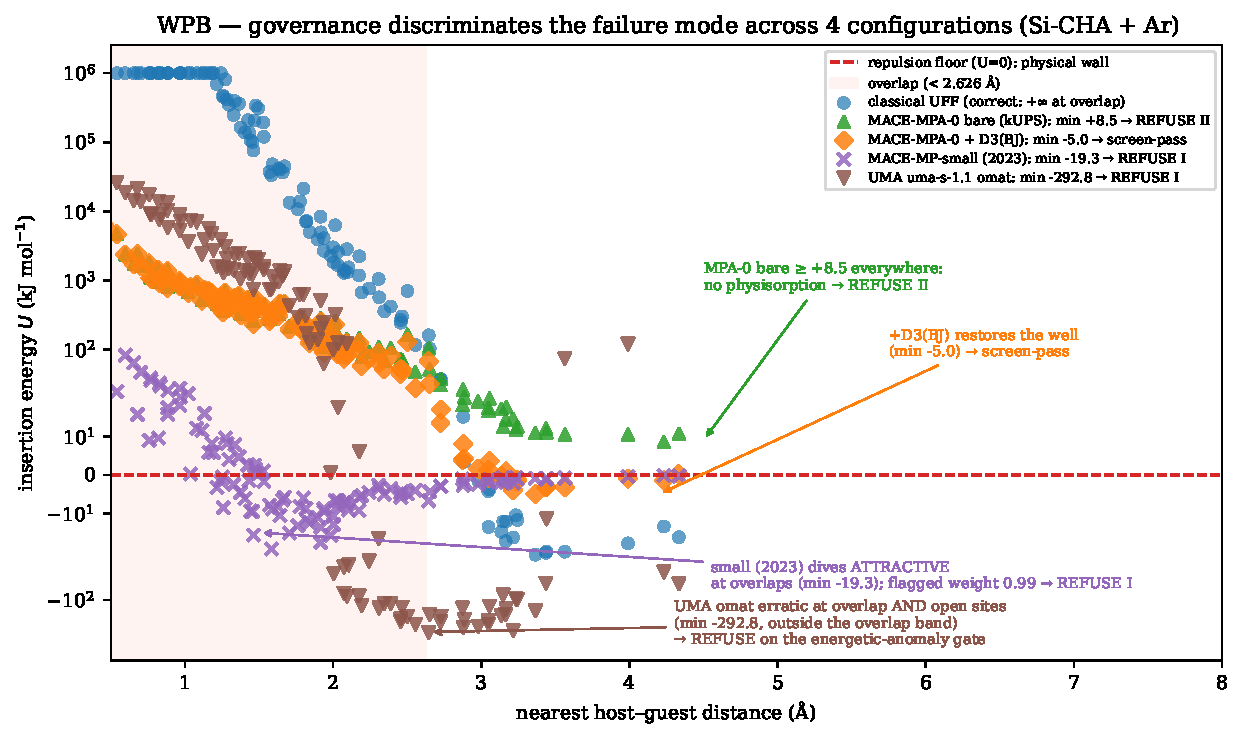
\includegraphics[width=0.95\linewidth]{f1_wpb_triptych.pdf}
\caption{WPB --- governance discriminates the failure mode across four configurations (Si-CHA + Ar).}
\end{figure}
\begin{figure}[h!]\centering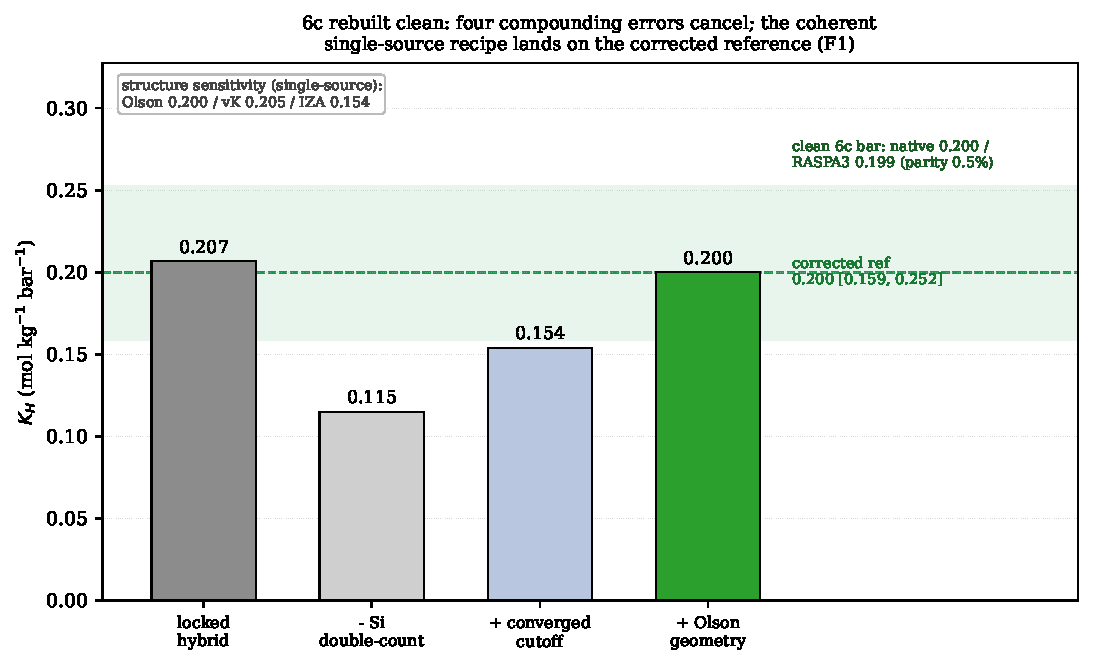
\includegraphics[width=0.80\linewidth]{fp_6c_cancellation.pdf}
\caption{Finding F1 --- branch 6c rebuilt clean. The originally-locked hybrid recipe (0.207) agrees with
the reference only as a fortuitous cancellation of four compounding errors; removing the silicon double-count, converging the
cutoff, and adopting Talu's calibration (Olson) geometry lands the coherent single-source recipe on the
corrected reference $K_H = 0.200$, cross-engine (native 0.200, RASPA3 0.199; parity 0.5\%). Values read
from \texttt{cancellation\_6c.json}.}
\end{figure}
\begin{figure}[h!]\centering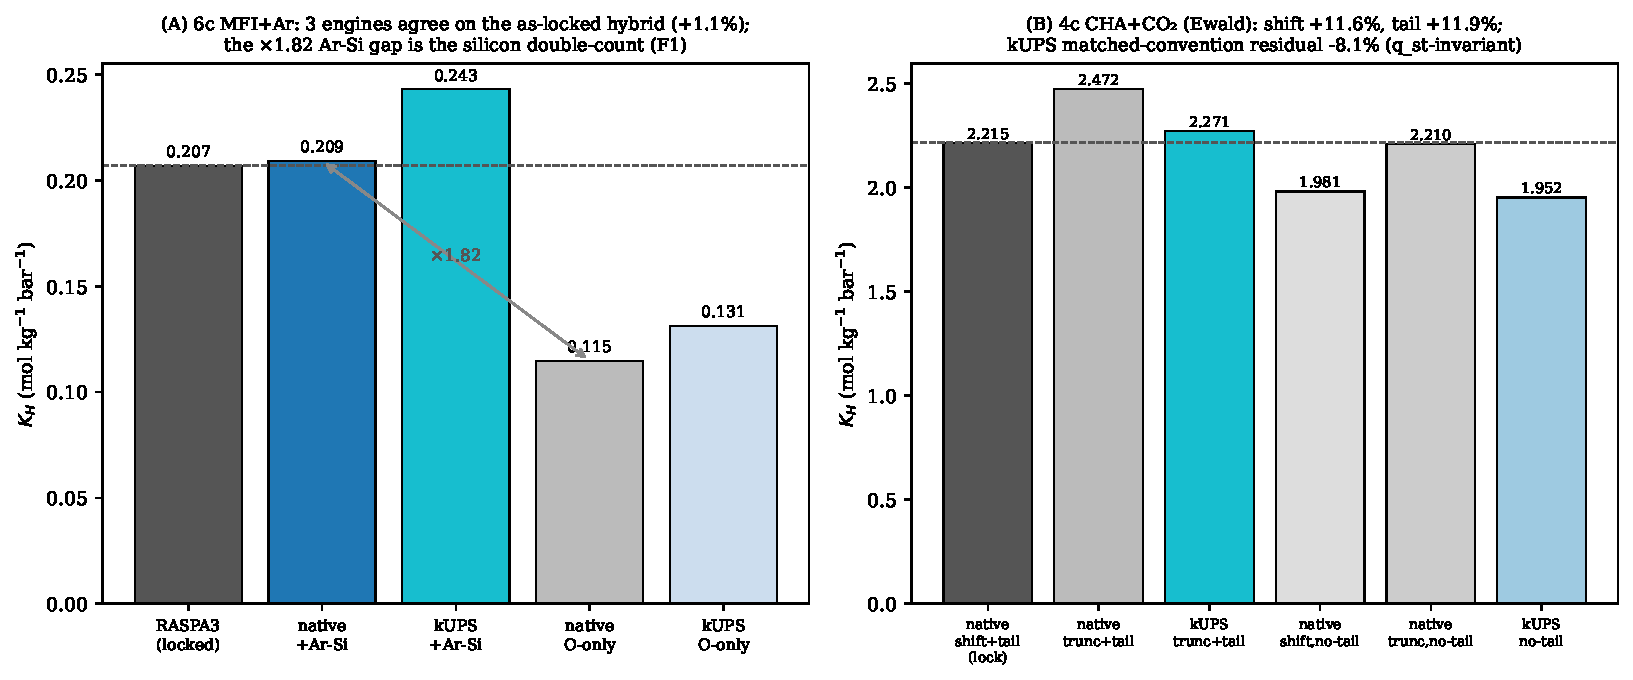
\includegraphics[width=0.98\linewidth]{fp_cross_engine_parity.pdf}
\caption{Cross-engine Widom parity: 6c three-way (native+Ar-Si reproduces RASPA3; the 1.8$\times$ gap to
O-only is the silicon double-count of Finding F1) and the 4c CHA+CO$_2$ convention matrix (shift / tail
toggles).}
\end{figure}
\FloatBarrier\clearpage
\begin{figure}[h!]\centering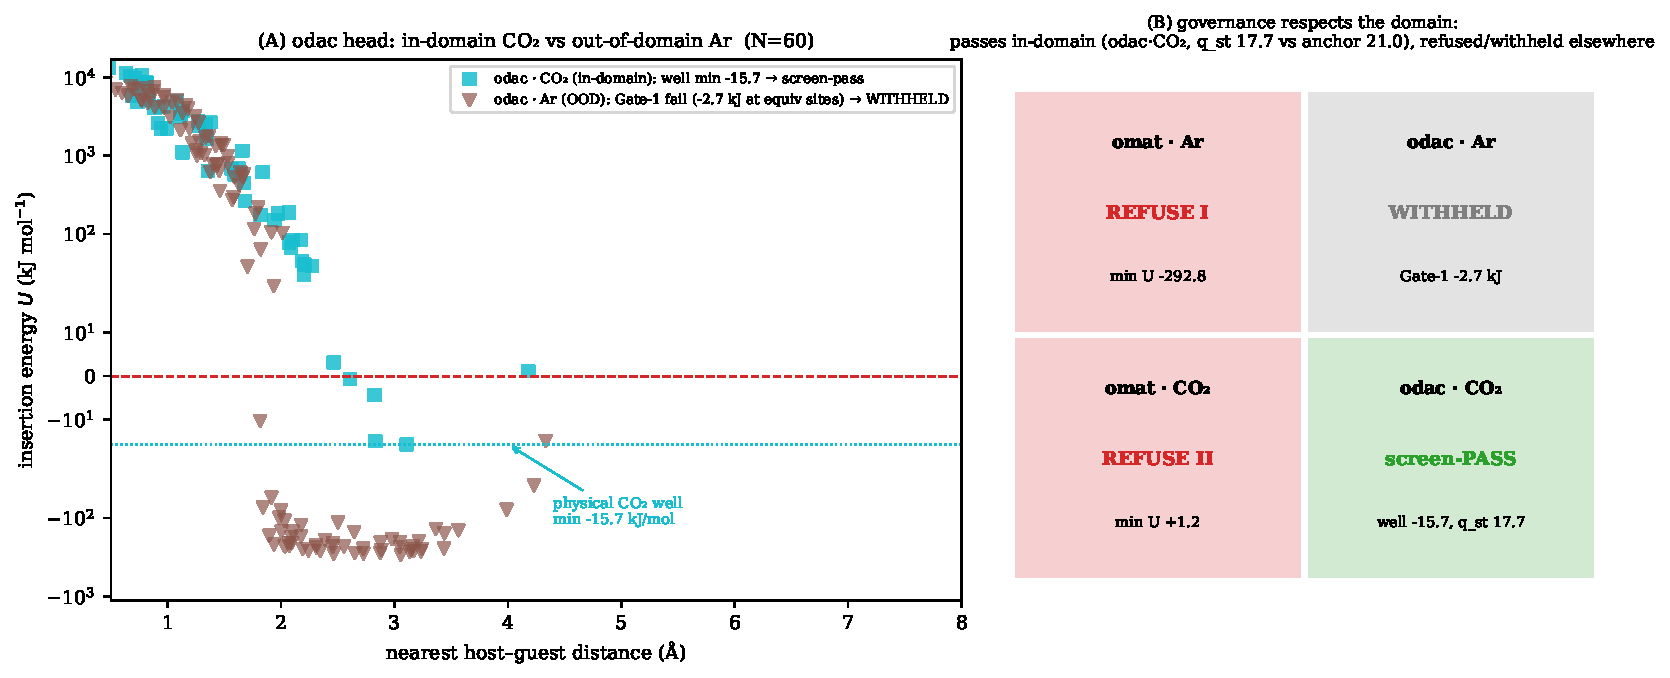
\includegraphics[width=0.98\linewidth]{f2_uma_domain.pdf}
\caption{Governance respects the training domain: the UMA odac head screen-passes in-domain on CO$_2$
and is WITHHELD out-of-domain on Ar; full task $\times$ system verdict matrix.}
\end{figure}
\begin{figure}[h!]\centering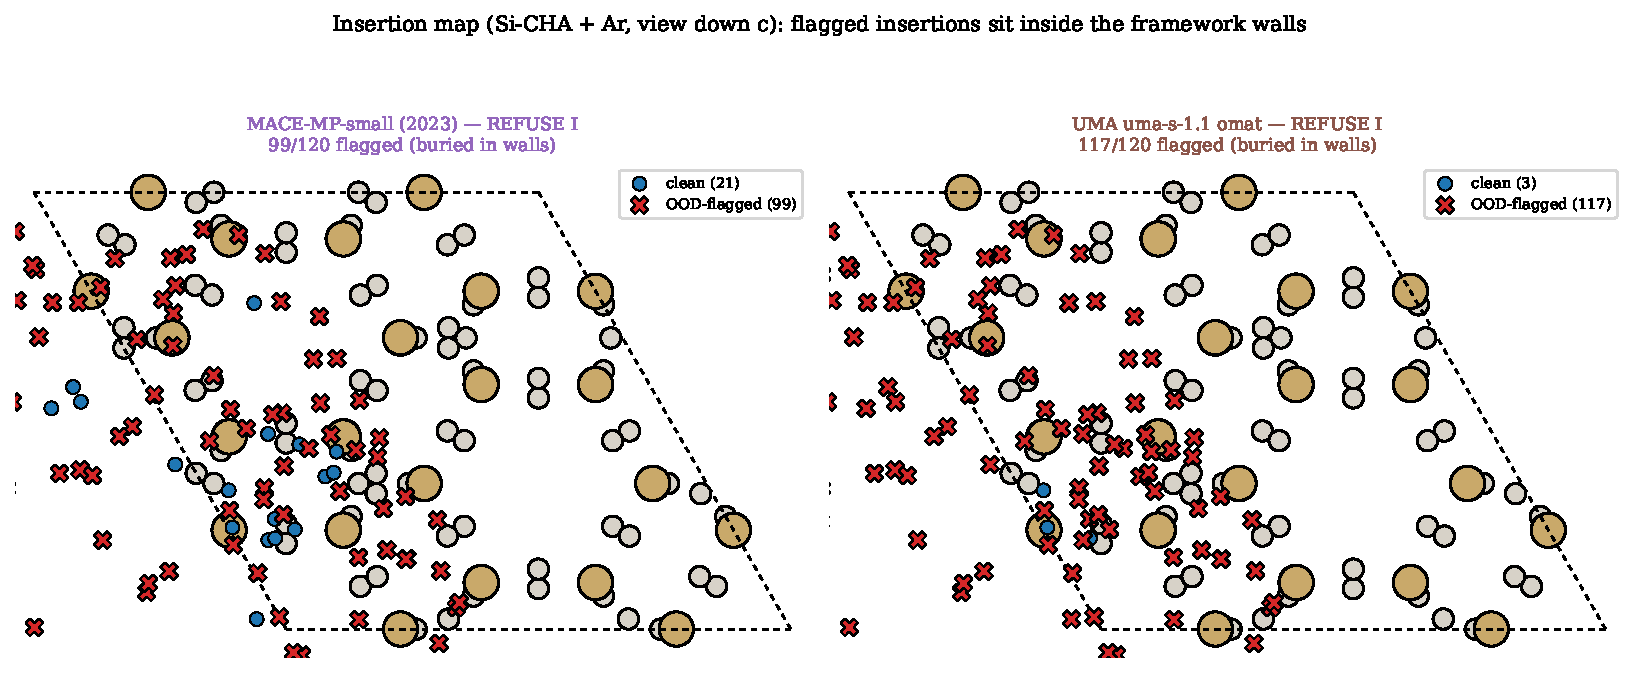
\includegraphics[width=0.95\linewidth]{f3a_insertion_map.pdf}
\caption{Where the spurious weight lives: flagged (OOD) insertions sit inside the framework walls.}
\end{figure}
\FloatBarrier\clearpage
\begin{figure}[h!]\centering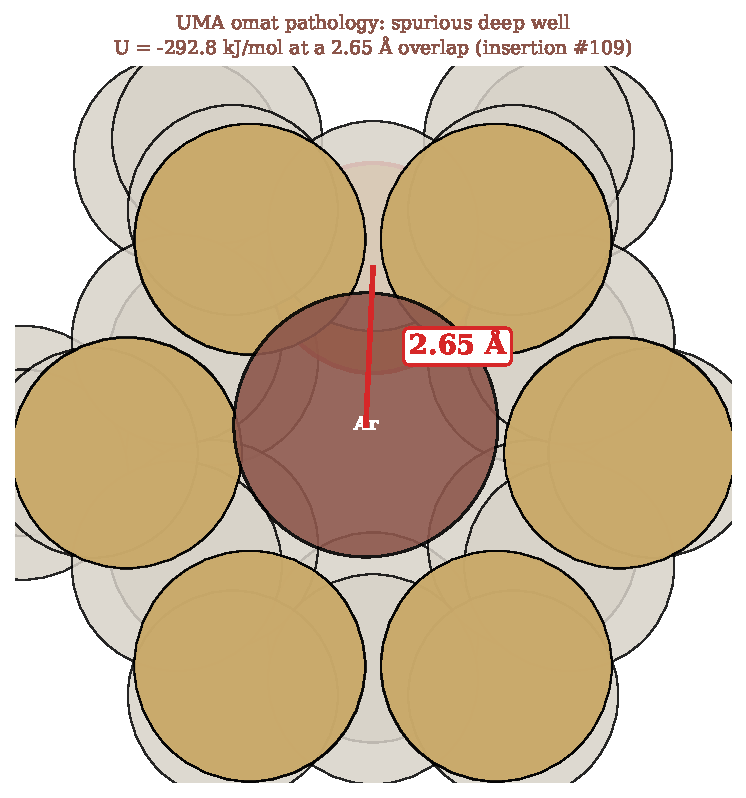
\includegraphics[width=0.62\linewidth]{f3b_pathology.pdf}
\caption{Pathology close-up: UMA's spurious deep well ($-292.8$ kJ/mol) at a 2.65 \AA{} atomic overlap.}
\end{figure}
\begin{figure}[h!]\centering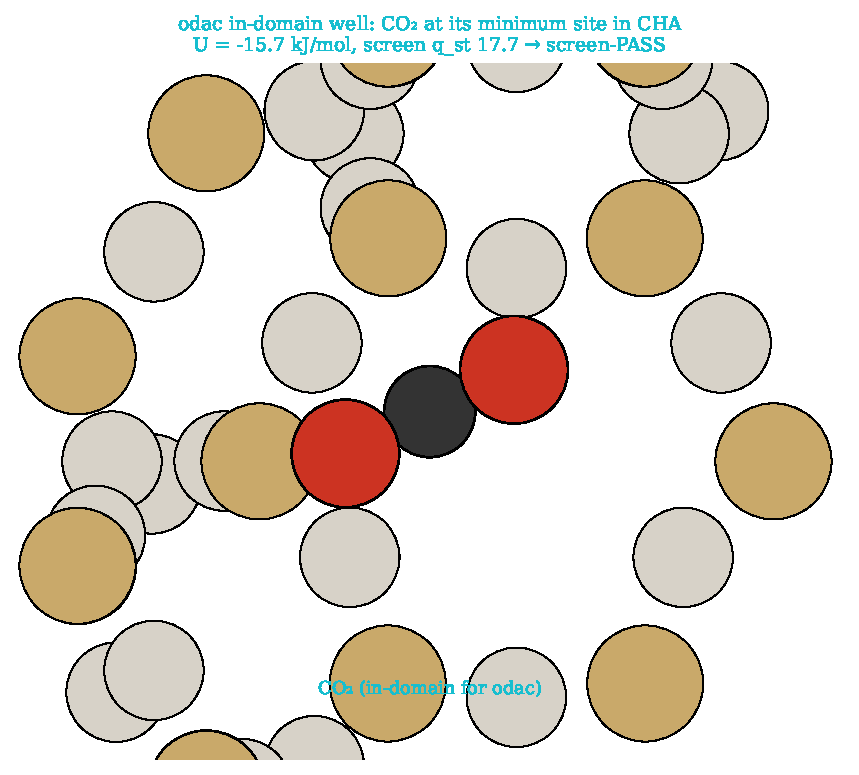
\includegraphics[width=0.62\linewidth]{f3c_indomain_well.pdf}
\caption{In-domain CO$_2$ well at the odac minimum-energy site (screen-pass).}
\end{figure}

\end{document}
